\section{$B$ mesons in proton-proton collisions}

In a proton-proton collision ($pp$ collision) many different particles are produced through the strong interaction.
When this includes the decay of a gluon into a $b\bar{b}$ pair, it can lead to the production of a $B$ meson.
$B$ mesons are composed of one $b$ quark and one of the $u/d/c/s$ quarks.
Relevant for this thesis are the uncharged $B$ mesons
\begin{align*}
    B^0 &= \bar{b}d \, , & \bar{B}^0 &= b\bar{d} \, , & B_s^0 &= \bar{b}s \, , & \bar{B}_s^0 &= b\bar{s} \, .
\end{align*}

At LHCb, a frequent goal is to analyse $B$ meson candidates in $pp$ collisions, often called the signal $B$.
This can be done by using information about the particles of the signal decay. 
Or it can be done by analysing all particles which are associated to the signal $B$.
The latter method is independent of the signal decay channel, and it is often used in flavour tagging algorithms at LHCb. 
A similar method is used in this thesis.
An example sketch of such an associated event is shown in \autoref{fig:ft_scheme}. 
This sketch excludes particles which are associated with the $pp$ collision event but not with the signal $B$.
Those particles are called the background of an event.

\begin{figure}
    \centering
    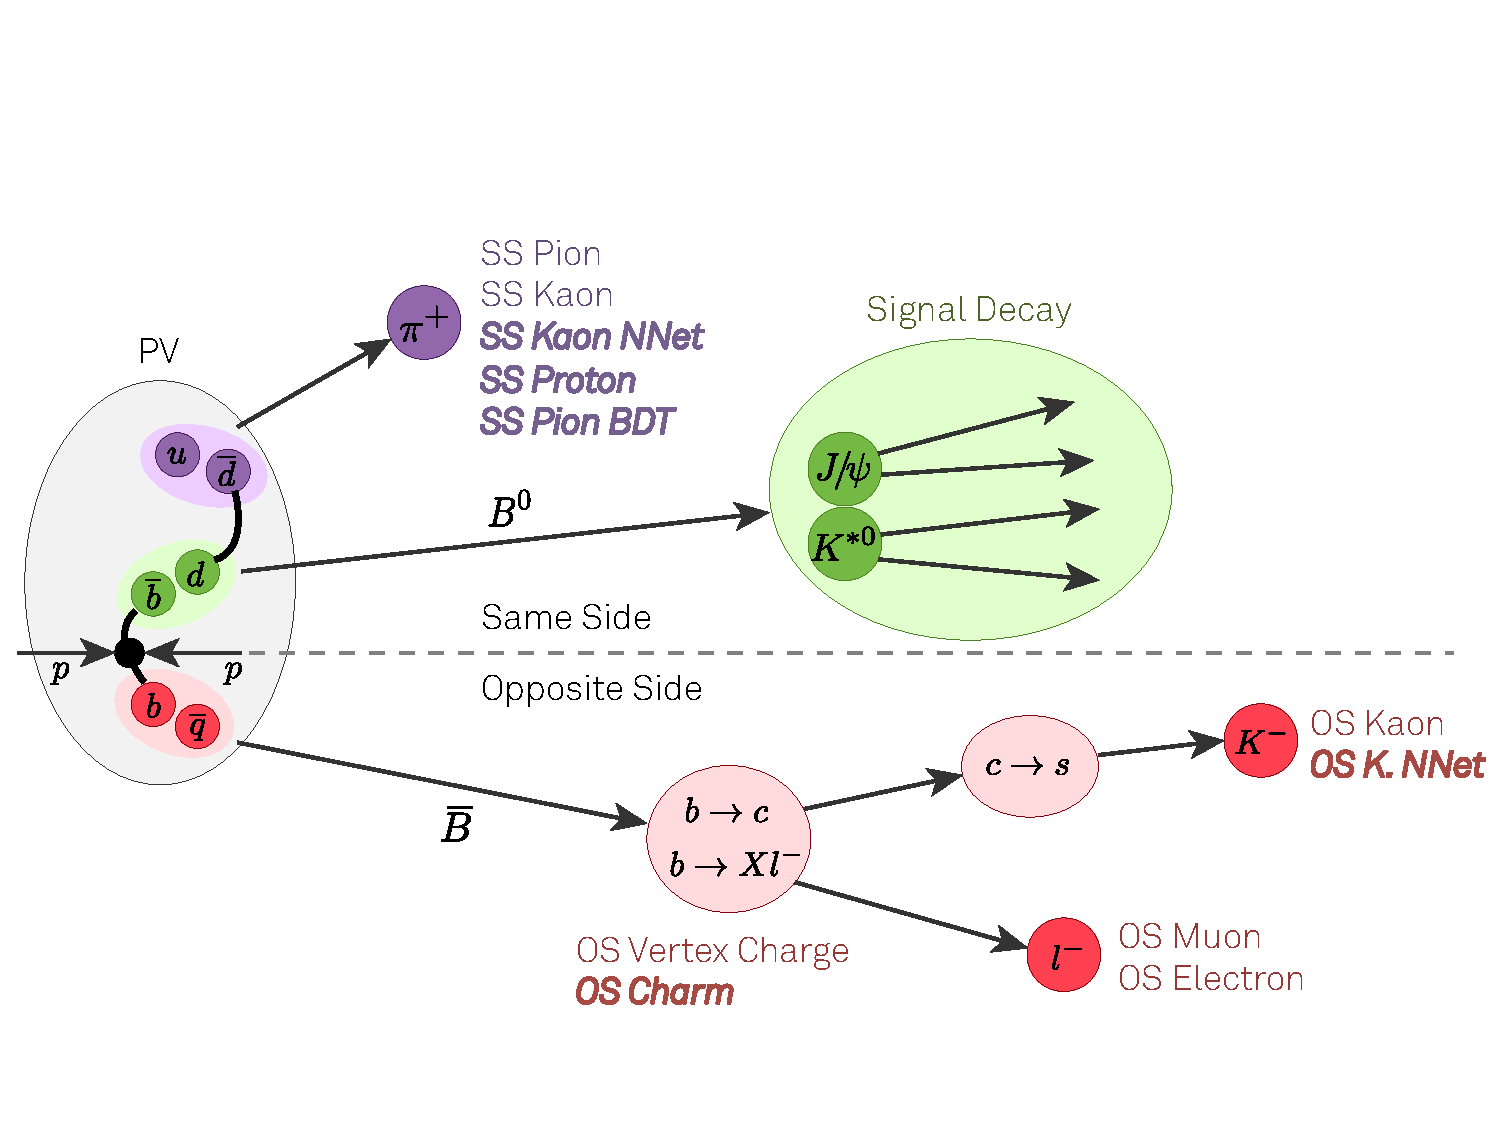
\includegraphics[width=\textwidth]{images/FlavourTaggingScheme.pdf}
    \caption{Schematic overview of the underlying principles of LHCb's flavour tagging algorithms \cite{ft_scheme}.}
    \label{fig:ft_scheme}
\end{figure}

The collision point of a $pp$ pair is called the primary vertex~(PV), and the decay point of the signal $B$ is called the secondary vertex~(SV).
Due to the high mass of $b$ quarks, an associated event can roughly be separated into two sides.
The same side~(SS) contains particles of the signal decay.
It also contains particles produced in association with the non-$b$ valence quark of the $B$ meson.
These particles are called the SS fragmentation.
The opposite side~(OS) contains all particles associated with the $b$ quark not in the signal $B$.
The combined information about the SS fragmentation and the OS allows the identification of the signal $B$ flavour.
